
% \documentclass[preprint]{IEEEtran}
\documentclass[preprint,12pt]{elsarticle}

\usepackage{color}
\usepackage{amsthm}
\usepackage{amsmath}
\newcommand{\beq}{\begin{equation}}
\newcommand{\eeq}{\end{equation}}
\newcommand{\sms}{\smallskip}
\newcommand{\ms}{\medskip}
\newcommand{\bs}{\bigskip}
\newcommand{\norm}[1]{\left\lVert#1\right\rVert}
\newtheorem*{problem}{Problem}
\newtheorem*{theorem}{Theorem}
\usepackage{graphicx}
\usepackage{lineno,hyperref}
\modulolinenumbers[5]
\newcommand\blfootnote[1]{%
  \begingroup
  \renewcommand\thefootnote{}\footnote{#1}%
  \addtocounter{footnote}{-1}%
  \endgroup
}
\bibliographystyle{elsarticle-num}
% \biboptions{compress}
% correct bad hyphenation here
\hyphenation{op-tical net-works semi-conduc-tor}
\journal{Mechanical Systems and Signal Processing}
% \journal{IEEE Transactions on Industrial Electronics}
\begin{document}
\begin{frontmatter}

\title{Novel method of informative frequency band selection for vibration signal using Nonnegative Matrix Factorization of spectrogram matrix}


\author[label3]{Jacek Wodecki \corref{cor1}}
\cortext[cor1]{Corresponding author, jacek.wodecki@pwr.edu.pl}
\author[label1]{Piotr Kruczek}
\author[label2]{Anna Bartkowiak}
\author[label3]{Radoslaw Zimroz}
\author[label4]{Agnieszka Wy{\l}oma{\'n}ska}

\address[label1]{KGHM Cuprum Ltd, Research and Development Centre, Sikorskiego 2-8, 53-659 Wroclaw, Poland}
\address[label2]{Institute of Computer Science, Wroc{\l}aw University, 50-383 Wroc{\l}aw, Poland, retired}
\address[label3]{Diagnostics and Vibro-Acoustic Science Laboratory, Faculty of Geoengineering, Mining and Geology, Wroclaw University of Science and Technology, Na Grobli 15, 50-421 Wroclaw}
\address[label4]{Faculty of Pure and Applied Mathematics, Hugo Steinhaus Centre, Wroc{\l}aw University of Science and Technology, Janiszewskiego 14a 50-370 Wroc{\l}aw, Poland}

% use for special paper notices
% \IEEEspecialpapernotice{(Invited Paper)}

% make the title area
% \maketitle

% As a general rule, do not put math, special symbols or citations
% in the abstract
\begin{abstract}
The problem of local damage detection in rotating machines is currently the highly important subject of interest in the field of condition monitoring. In the literature one can find many different strategies. One of the most common approaches is the vibration signal analysis aiming at informative frequency band selection. In case of simply structured signals classic methods (e.g. spectral kurtosis) are sufficient and return clear information about the damage. However, in real-world cases the signal is usually much more complicated. Indeed, such signals consist of many different components, for instance: damage-related cyclic impulses, heavy-tailed background noise etc. Hence, there is a growing need for robust damage detection methods. In this paper a novel method of informative frequency band selection is proposed. It utilizes the approach of Non-negative Matrix Factorization applied to time-frequency signal representation. The described algorithm is evaluated using simulated signal containing several different components, that resembles real-life vibration signal from copper ore crusher, as well as real-life signal measured on the crusher. Using the obtained structure of informative frequency band it is possible to filter particular components out of the original signal.
\end{abstract}

% no keywords
% \begin{IEEEkeywords}
\begin{keyword}
nonnegative matrix factorization, filtration, vibration measurement, time-frequency representation, spectrogram
% \end{IEEEkeywords}
\end{keyword}

\end{frontmatter}

\linenumbers
\section{Introduction}
% \blfootnote{Elements of this methodology were already presented at IEEE SDEMPED 2017 conference \cite{wodecki2017nonnegative} with regard to using only simulated data. In presented article authors extend the research to the analysis of real data as well.}

Condition monitoring is highly important part of the maintenance of rotating machinery. One of the most common approaches is based on the analysis of the vibration signal. Unfortunately, in most cases real-life industrial signals reveal too complicated structure to be analyzed with simple time domain methods \cite{randall2011rolling}. Due to nonstationary character of the signal, one of the most popular approaches is using different representations of data, mainly time-frequency domains or bi-frequency representation, i.e. spectral coherence \cite{randall2011rolling}. Recent methods for time-frequency analysis of rotating machinery are illustrated in \cite{feng2013recent}. 
There are many works published on cyclostationary analysis of vibration signals in gearboxes or bearings, mostly driven by Antoni \cite{Borghesani2017,antoni2016info,antoni2019, abboud2019}.We would like to highlight importance of simultaneous observation of impulsiveness and cyclicity or design of new condition indicators. Cyclostationary approach seems to be the most powerful in condition monitoring applications, however, in our opinion, the problem of non-Gaussian noise still required further studies.

Of course, there are also different techniques used for such analyses. Interestingly, stochastic modelling methods are also powerful in case of condition monitoring. For instance, application of Schur filter is presented in \cite{Makowski2014130} and autocorrelation and partial autocorrelation functions are used in \cite{zak2014novel}. Furthermore, in \cite{kruczek2017cyclic} the application of periodically varying filter for fault indication is presented.
The detection of damage can be also performed with selection of informative frequency band (IFB) \cite{obuchowski2014selection,antoni2006spectral,combet2009optimal}. 
It stands for the frequency band where information about damage exsists and it is relatively easy to identify (Signal to Noise Ratio is high enough to detect damage). Local damage is manifested by cyclic impulsive contribution in the measured signal. In practical applications these impulses are not visible or easily identifiable in the raw signal due to high level of noise. However, noise is present at any frequency (whole band is affected), while damage-related energy is typically located at resonance area. Prefiltering of raw data at some unknown informative frequency band (called IFB) significantly improves signal-to-noise ratio (SNR) and allows to detect damage.

 
The most classical approach for IFB identification is spectral kurtosis, which indicates the kurtosis for each frequency band in time-frequency representation of the signal. In case of simple signal, which does not contain many different components spectral kurtosis is sufficient. On the other hand, in case of the machine working in harsh condition the condition monitoring is more complicated because of the presence of multiple impulsive components with overlapping frequency bands. Thus, the classical methods fail and new approach should be proposed. One of the possible solution is an application of heavy tailed distribution, namely $\alpha$-stable distribution can be incorporated for informative band selection \cite{zak2016data}. Moreover, in case of the early stage of the damage another distribution can be applied. Indeed, the tempered stable distribution reveals an ability to detect smaller impulses \cite{wylomanska2016application}. In case of mining industry the working condition is harsh, there are many different sources of high energy noise. The contamination of vibration signal is high and cyclic impulses are hidden in the background noise. Therefore, the condition monitoring of the mining machinery is especially challenging \cite{bartelmus2014object}. The example of such machine is copper ore crusher. During the mechanical crushing process of oversized rock pieces high non-cyclic impulses are generated. The signal recorded on such machine was analysed in \cite{wylomanskaimpulsive}. The regime switching method for impulsive noise cancellation was used. As a result the signal component related to cyclic impulse was obtained. 

Main idea of presented methodology is based on extracting underlying information from the mixture of different behaviors. To achieve desired results, nonnegative matrix factorization (NMF) is used. In the literature it has been shown that NMF is a useful tool in data analysis and clustering \cite{cichocki2009nonnegative, zdunek2008data, wang2013nonnegative, lee1999learning, lee2001algorithms, he2011symmetric}.

A variant of this method has been already considered in \cite{wodecki2017local}, where the application of (NMF) to the time-frequency representation of the signal. In that case so-called \emph{encoding matrix} produced by NMF was used to classify spectra vectors along the time dimension. In this paper a different approach is proposed, where authors factorize the spectrogram matrix, however so-called \emph{base matrix} is used. As a result the filter characteristic is designed, that allows to isolate the damage component. Method is deployed for the signal, which contains cyclic and high energy non-cyclic impulses. It is expected that each signal component can be extracted from original waveform. 


The rest of the paper is structured as follow. In Section \ref{sec:methodology} the proposed methodology is introduced, the theory of NMF is recalled and the flowchart is presented. The application of the algorithm for simulated data is contained in Section \ref{sec:sim data}. In section IV the respective considerations are applied for real-life data, namely for ore crusher. Finally, the conclusions are presented in the last Section.

\section{Methodology}
\label{sec:methodology}
\subsection{Standard NMF with Euclidean objective}

Let $\bf{V}_{n\times m}$ denote an observed matrix {\bf  V} of size $(n\times m)$ with non-negative elements. For such data matrix ${\bf V}$, Lee and Seung  proposed a factorization into two components \cite{lee2001algorithms}:

\beq\label{V1} {\bf V}_{n\times m}\simeq
      {\bf W}_{n\times r}*{\bf H}_{r\times m}. \eeq
      
All elements of the sought matrices ${\bf W}$ and ${\bf H}$ also have to be
non-negative, which is expressed by the constraints
\begin{align*}
    &v_{ij}\ge0,~~w_{ik}\ge 0,~~ h_{kj}\ge 0,\\
    &~~i=1, \dots, n; ~j=1,\dots, m;
                ~~k=1,\dots,r.
\end{align*}

The parameter $r$ is supposed to satisfy the inequality: $r~<= min(n,m)$.
In the following, the parameter \emph{r} will represent the expected number of components in the signal.


Concerning the data matrix \textbf{V} appearing in Eq. (\ref{V1}), the authors \cite{lee1999learning} consider it as the 'visible' (hence the '\textbf{V}' letter) data matrix. \textbf{V} contains in its columns \textit{m} 'objects' (like face images, documents, etc) under investigation. Each 'object' is characterized by \textit{n}
variables alias traits (like pixels for face images or words for documents).

Formula \ref{V1} says  that the original data matrix \textbf{V} is
approximated by the product of following real-valued lower rank matrices: \emph{base matrix} ${\bf W}_{n\times r}$ and \emph{encoding matrix} ${\bf H}_{r\times m}$  which have jointly less elements than ${\bf V}$, i.e. the following inequality holds:
('$< <$' in (\ref{r1}) means: much smaller)

\begin{equation}\label{r1}
    (n+m)*r<\hspace{1pt}< n*m . 
\end{equation}

If truly formula (\ref{V1}) holds, which means, {\bf V} is well
approximated by the product {\bf W}*{\bf H}, then we may conclude that the
analyzed data matrix {\bf V} may be efficiently stored (and analyzed)
using only about (n+m)*r instead of n*m data elements.

To approximately factorize $\textbf{V}\simeq{\textbf{W}*\textbf{H}}$, one should define cost function that quantifies the approximation quality. Lee and Seung proposed three possibilities for cost function: Euclidean distance, divergence and Poisson error. One of the most common and useful measures, also used in presented implementation, is the square of the Euclidean metric:

\beq  
\norm{\textbf{V}-\textbf{WH}}^2
\eeq

The function $\norm{\textbf{V}-\textbf{WH}}^2$ is convex in terms of \textbf{W} only or \textbf{H} only, but not convex in both of them together. Hence, it is typically impossible to find global minima. However, many optimization techniques can be applied to obtain them.
Perhaps the simplest one to implement is gradient descent, but its convergence is not very fast. Some other methods such as conjugate gradient converge quicker, at least in the neighbourhood of local minima, but are more complex to implement.

It has been determined by Lee and Seung that the following multiplicative element-wise update formulae (for practical implementation presented in matrix forms by Hoyer \cite{hoyer2004non}) are fast to compute and easy to implement for minimizing the cost function:\newline

\begin{theorem}
The Euclidean metric $\norm{\textbf{V}-\textbf{WH}}$ is non-increasing under the update rules 
% \begin{equation}
%     H_{\alpha\mu} \leftarrow H_{\alpha\mu}\frac{(W^TV)_{\alpha\mu}}{(W^TWH)_{\alpha\mu}} \quad
%     W_{i\alpha} \leftarrow W_{i\alpha}\frac{(VH^T)_{i\alpha}}{(WHH^T)_{i\alpha}}.
% \end{equation}
\begin{equation}
\begin{array}{ll}
     &\mathbf{H} \leftarrow \mathbf{H}\otimes(\mathbf{W^TV})\oslash
(\mathbf{W^TWH}) \quad  \\
     & \mathbf{W} \leftarrow \mathbf{W}\otimes(\mathbf{VH^T})\oslash(\mathbf{WHH^T}).
\end{array}
\end{equation}
\end{theorem}

where $\oslash$ denotes elementwise division and $\otimes$ denotes the elementwise multiplication \cite{lee2001algorithms}. Update of both matrices need to be performed simultaneously. Matrices \textbf{W} and \textbf{H} are also being renormalized by the norms of rows of matrix \textbf{H} for constant energy of the clusters. In principle, normalizaton is performed by the columns of matrix \textbf{W} \cite{cichocki2009nonnegative}:

\begin{equation}
    \mathbf{W} \leftarrow \mathbf{WD_W},
\end{equation}

where 
\begin{equation}
    \mathbf{D_W}=diag\left(\norm{w_1}^{-1},\norm{w_2}^{-1},\dots \norm{w_J}^{-1} \right), 
\end{equation}
in our case input matrix \textbf{V} is transposed relative to the derivation described in \cite{cichocki2009nonnegative}, so output matrices of NMF algorithm are inverted in their functionality. Hence, in practice normalization is performed iteratively by the rows of matrix \textbf{H}, that rewritten for individual rows of matrix \textbf{H} and columns of matrix \textbf{W} presents itself as follows:

\begin{equation}
    W_{k} \leftarrow \frac{W_{k}}{\norm{H_{k}}}
    \quad
    H_{k} \leftarrow \frac{H_{k}}{\norm{H_{k}}},
\end{equation}
where $\norm{H_{k}}$ is an Euclidean norm of the vector $H_{k}$.

\subsection{Scope of the diagnostic algorithm}

\begin{figure}[!ht]
\centering
\includegraphics[width = 0.5\textwidth]{figs3/block.png}
\caption{Flowchart of the proposed methodology}
\label{fig: block}
\end{figure}

% \textcolor{red}{Selektory zostana lepiej opisane przez AW}

Functional flowchart of the proposed methodology is presented in Fig. \ref{fig: block}. Firstly, signal has to be transformed into a time-frequency domain. For such transformation spectrogram has been chosen. Short-time Fourier transform (STFT), which for discrete data $x[0], x[1], ... , x[N-1]$ is given by the formula \cite{allen1977short}:

\begin{equation}
    \textrm{STFT}(k,g)=\sum_{f=0}^{L-1}x[g+f]w[f]e^{-j2\pi kf/N},
\end{equation}
where $0\leq k \leq N-1$ is frequency bin, $g$ is time point and  $w[.]$ is the window of length $L$. One can observe that, in STFT for each time point the Fourier Transform is calculated using FFT. Furthermore, the spectrogram is squared absolute value of the STFT:

\begin{equation}
\textrm{Spec}(k,n)=|\textrm{STFT}(k,g)|^2.
\end{equation}

% \textcolor{blue}{(RZ:akapit do podmiany - ten skasowac)}

% After that NMF algorithm is applied to extract spectral information about different types of processes occurring in the signal. \textcolor{red}{Thus, the transposed spectrogram matrix is provide to NMF algorithm as input matrix} \textbf{V}. As a result, $r$ \textcolor{red}{IFB} selectors are obtained as column vectors of base matrix {\bf W}, where $r$ is the predefined expected number of classes of processes. 


Considering time frequency map as nonnegative data matrix we apply NMF to factorize spectrogram. In this context NMF is used as clustering tool - we want to group spectral vectors  $\textrm{Spec}[f,\Delta t[i]]$, where $f$ denotes full Nyquist frequency domain for given data. Obtained spectrogram matrix $Spec$ will serve as matrix $\mathbf{V}$ for NMF factorization (see Eq. \ref{V1}). To perform the factorization, we define the value $r$ as the rank of factorization. We perform NMF factorization to obtain the matrix \textbf{W} that will be composed of \textit{r} vectors - related to clusters - that contain description of spectral content of each cluster $i=1 \dots r$. Each column vector of \textbf{W} is considered as averaged spectral density and can be used as filter characteristic (also named \emph{selector}).

Finally, input signal is filtered with FIR filter, where given selector is used as filter frequency response \cite{alan1989discrete}. At the end, envelope spectra of obtained signals are calculated to inspect fundamental and harmonic frequencies of the components \cite{randall2011rolling}. Additionally, IFB can be presented as a frequency band for which the desired selector is the strongest of the whole bank.

\section{Simulated data analysis}
\label{sec:sim data}
\subsection{Problem formulation and description of simulated data}
In this article the vibration signals acquired on the heavy duty copper ore crusher are analyzed. This machine is used to reduce the size of the huge pieces of ore. In this industrial process the background noise is highly impulsive and non-cyclic. It is related to the material flow through the crusher (pieces of ore hitting housing of the crusher) and crushing process. In such case the signal of interest, containing cyclic information about the fault, is invisible  because of high contamination. Furthermore, for signal with the non-cyclic highly energetic impulses the classical approaches based on impulsivity cannot be applied. It is proposed to apply the NMF to extract all of the signal components separately. 

In the first part the simulated signal, which resemble the copper ore crusher is going to be analyzed. Therefore, we simulate three types of signals:

\begin{enumerate}
    \item Component consisting of cyclic impulses, called Signal of Interest (SOI) with cyclic frequency equal to 40 Hz and carrier frequency around $2500-3500$ Hz (Fig. \ref{fig:schemat sygnal} a);
    \item Gaussian noise - accompanying the SOI, that has mean equal 0 and variance 0.2 (Fig. \ref{fig:schemat sygnal} b);
    \item Impulsive non-Gaussian noise with center frequency equal to 5000 Hz, but varying bandwidths (Fig. \ref{fig:schemat sygnal} c).
\end{enumerate}

\begin{figure}[ht!]
    \centering
    \includegraphics[width = 0.6\textwidth]{figs3/sym_signal_components.png}
     \caption{ Components of the simulated signal: a) Component consisting of cyclic impulses (SOI), b) Gaussian noise, c) Impulssive non-Gaussian noise with energy significantly higher than all remaining components}.
    \label{fig:schemat sygnal}
\end{figure}


Combination of those signals is supposed to imitate the operation of ore crusher. SOI simulates local damage in rolling bearing of the crusher, Gaussian noise is related to the measurement noise and bearing operation in healthy condition, and impulsive non-Gaussian noise simulates random events of falling rocks or crushing process. Every impulsive signal is composed of individual impulses generated by MATLAB function \emph{gauspuls}. This dataset was previously used in \cite{wylomanskaimpulsive}, where more precise description can be found. Thus, observed signal is composed of three signals in such a way that SOI is effectively hidden in the Gaussian noise and is not directly visible. In \cite{wylomanskaimpulsive} authors proposed novel methodology to identify the impulsive non-Gaussian component and remove it from the signal. The  advanced and quite complicated Hidden Markov Regime Switching Model was used. 



\subsection{Results for simulated data}

Time series of simulated  signal is presented in Fig. \ref{fig: input}. This data has been already addressed in \cite{wylomanskaimpulsive}. Spectrogram is computed for parameters presented in Table \ref{tab:tab1}. One can observe several strong, non-cyclic excitations emerging from the noise, but no cyclic impulses are visible. Even on spectrogram they are not very obviously noticeable (see Fig. \ref{fig: spectrogram}).
\begin{table}[ht!]
    \centering
    \caption{Parameters of spectrogram}
  \begin{tabular}{|l|l|}
    \hline
    \textbf{Parameter} & \textbf{Value} \\ \hline
         Signal length & 1 second (25000 samples) \\ \hline
         Sampling frequency & 25000 Hz \\ \hline
         Window & Hamming, 256 samples \\ \hline
         Overlap & 220 samples \\ \hline
         FFT points & 512 samples \\ \hline
         Spectrogram size &  $257 \times 688$\\
         
    \hline
    \end{tabular}
    \label{tab:tab1}
\end{table}

\begin{figure}[!ht]
%\vspace{-10pt}
\centering
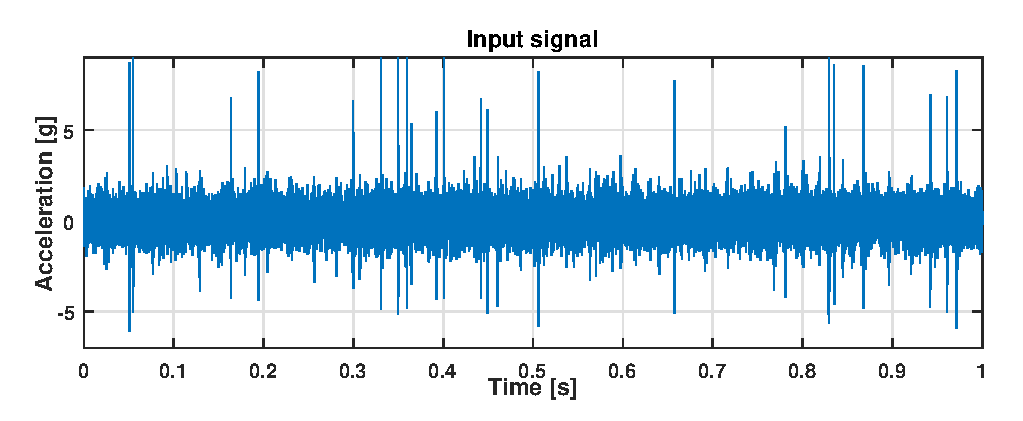
\includegraphics[width = 0.8\textwidth]{figs3/input_sig.eps}
\caption{Simulated input signal}
\label{fig: input}
\end{figure}

\begin{figure}[!ht]
\centering
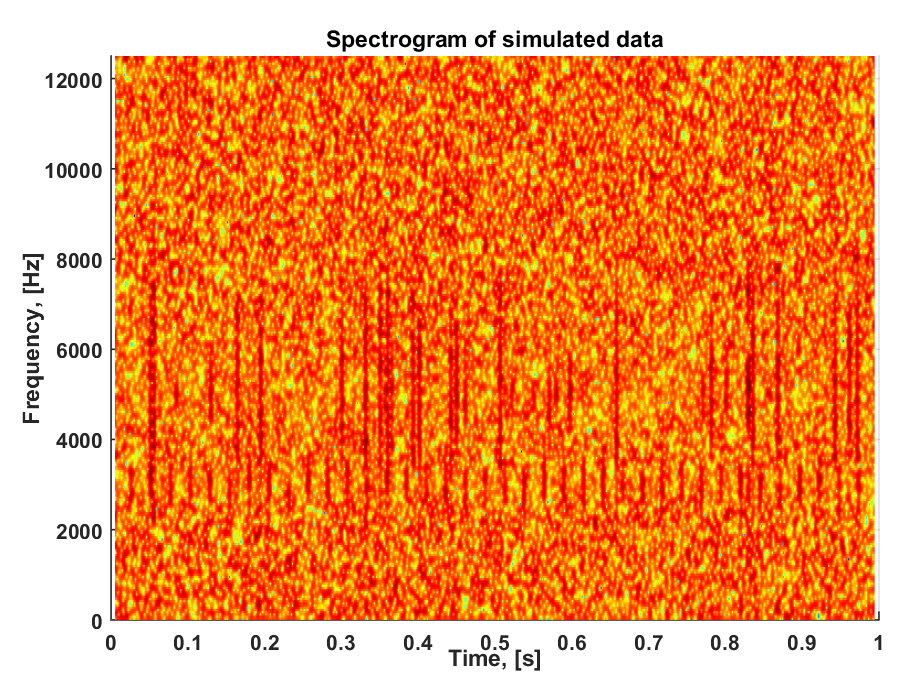
\includegraphics[width = 0.7\textwidth]{figs3/input_spec.eps}
\caption{Time-frequency representation of the input signal}
\label{fig: spectrogram}
\end{figure}

As a next step, spectrogram matrix \textbf{V} is provided as input for NMF algorithm, which differentiates spectral profiles of previously described processes (see Fig. \ref{fig: selmat}). Since the process is artificially designed, the exact number of components is known. Hence, number of desired classes for NMF algorithm has been set to 3. Based on the visual inspection of the spectrogram matrix, one can recognize that second cluster describes spectrum of cyclic impulsive component, and third component is responsible for the non-cyclic process.

\begin{figure}[!ht]
\centering
\includegraphics[width = 0.7\textwidth]{figs3/selector_matrix.png}
\caption{Matrix W containing r=3 IFB selectors obtained by NMF from simulated data}
\label{fig: selmat}
\end{figure}

Selectors used as transfer functions for the filtration step are presented in Fig. \ref{fig: selplots}. According to blue curve, signal component related to cyclic impulses is informative for frequencies around 3~kHz. It could be considered as informative band. On the other hand the red curve has the highest values for frequency ranges 0-2kHz and 7.5kHz-12.5kHz, however the level is almost flat. Finally, the component related to non-cyclic impulses (orange curve) has a bit higher amplitudes for frequency range 3.5Hz-7.5kHz than for other frequencies. It is worth mentioning that, blue curve amplitude is significantly higher than for other spectral profiles.

\begin{figure}[!ht]
\centering
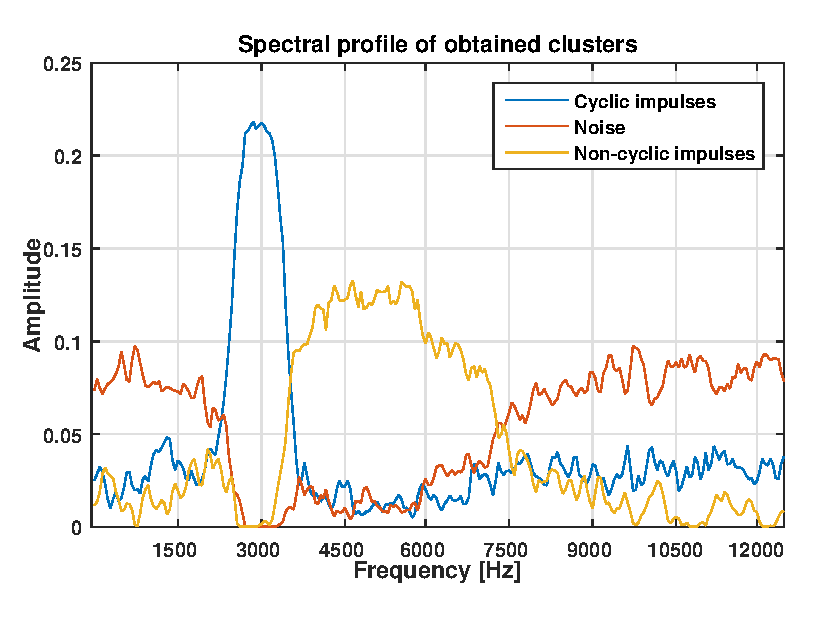
\includegraphics[width = 0.7\textwidth]{figs3/selector_plot.eps}
\caption{Spectral profiles (selectors) of obtained clusters for simulated signal}
\label{fig: selplots}
\end{figure}

Input signal (Fig. \ref{fig: outplots} a) has been filtered with two selectors extracting non-cyclic and cyclic components (Fig. \ref{fig: outplots} b and c respectively). Obtained signals carry information about random impacts being natural behavior of this type of machines, and cyclic impulsive process that denotes detected local damage. It is worth mentioning that, the operation of filtration reduce the energy of the signal because filter characteristic is not normalized. Therefore, the data after the filtration has smaller amplitude.

\begin{figure}[!ht]
\centering
\includegraphics[width = 0.7\textwidth]{figs3/output_plots.png}
\caption{Results of filtration for simulated signal: a) original signal, b) non-cyclic impulses, c) cyclic impulses}
\label{fig: outplots}
\end{figure}

\begin{figure}[!ht]
\centering
\includegraphics[width = 0.7\textwidth]{figs3/output_specs2.png}
\caption{Envelope spectra of the results for simulated signal: a) original signal, b) non-cyclic impulses, c) cyclic impulses}
\label{fig: outspecs}
\end{figure}



In addition, quality and clarity of obtained components can be evaluated using envelope spectra (see Fig. \ref{fig: outspecs}), which are commonly used for detecting periodicity of impulses \cite{randall2011rolling}. This is a powerful method for fault detection for rolling elements bearings \cite{randall2011rolling}. Spectrum of input signal (panel a) provides no conclusive information about the damage. Although there are several visible peaks in the spectrum, their presence and they have no physical meaning. Envelope spectrum of non-cyclic component (panel b) looks random, which is expected effect because of randomness of impulses' bandwith and position in time domain. Finally, envelope spectrum of cyclic component (panel c) provides unquestionable series of peaks at fundamental and harmonic frequencies related to local damage (in this case 40 Hz and its multiples). IFB determined for this component spans the frequencies between 2344 Hz and 3515 Hz of the carrier.



\section{Real-life data analysis of copper ore crusher}

In this section authors present the application of proposed extraction method to the real-life vibration signal from copper ore crusher operating in mining industry. Since there was no available signal from faulty crusher (all machines turned out to be in good technical condition), an artificial damage has been introduced to healthy signal to simulate cyclic damage. Component has been introduced in a way that it is not directly visible in the time series (Fig. \ref{fig: input2}) or in the envelope spectrum (Fig. \ref{fig: widma2} top).

\begin{figure}[!ht]
\centering
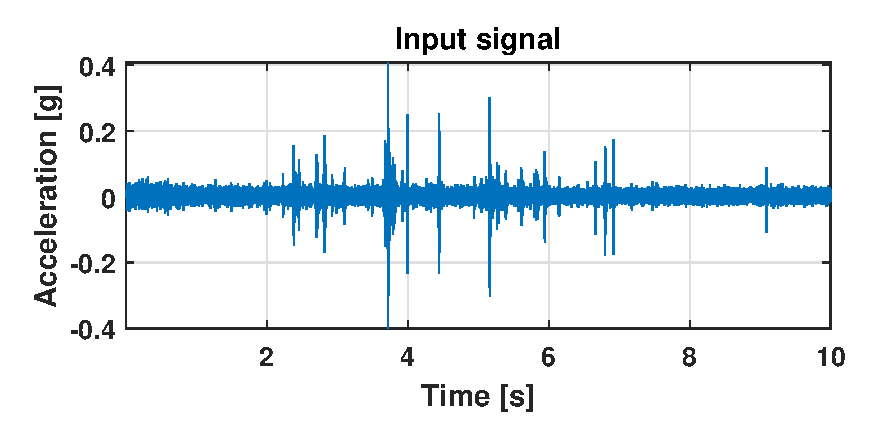
\includegraphics[width = 0.8\textwidth]{figs3/input.eps}
\caption{Input vibration signal of the ore crusher}
\label{fig: input2}
\end{figure}

In Fig. \ref{fig: input2} input vibration signal is presented. Time series reveals numerous high-energy wideband impulses being the result of rocks falling into the machine. On the other hand, cyclic damage component is barely noticeable above the noise floor. Parameters of spectrogram calculated for this dataset are presented in Table \ref{tab:tab2}.


\begin{table}[ht!]
    \centering
    \caption{Parameters of spectrogram}
  \begin{tabular}{|l|l|}
    \hline
    \textbf{Parameter} & \textbf{Value} \\ \hline
         Signal length & 10 second (250000 samples) \\ \hline
         Sampling frequency & 25000 Hz \\ \hline
         Window & Hamming, 256 samples \\ \hline
         Overlap & 215 samples \\ \hline
         FFT points & 512 samples \\ \hline
         Spectrogram size & $257 \times 6404$ \\
         
    \hline
    \end{tabular}
    \label{tab:tab2}
\end{table}


Time-frequency representation of data is presented in Fig. \ref{fig: spec2}.

\begin{figure}[!ht]
\centering
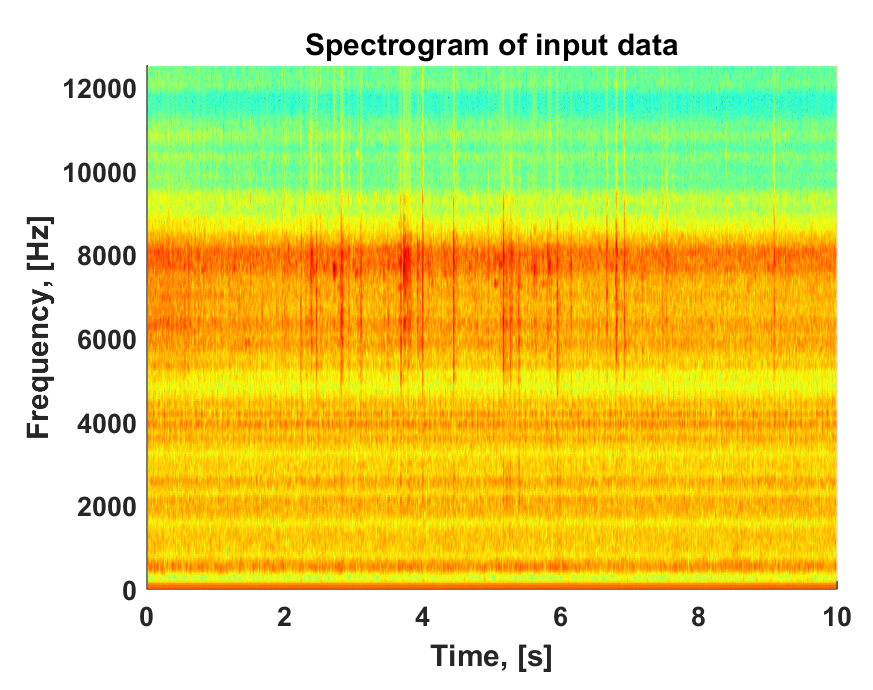
\includegraphics[width = 0.7\textwidth]{figs3/spec.eps}
\caption{Time-frequency representation of the input signal from the ore crusher}
\label{fig: spec2}
\end{figure}

One can notice heavy impulses across almost entire frequency dimension, while the cyclic component is weak and located in the frequency band roughly between 2200 Hz and 4800 Hz. Hence real signal is more complicated in its structure than the simulated one, the optimal amount of clusters had to be evaluated. According to Silhouette criterion \cite{kaufman2009finding,rousseeuw1987silhouettes}, commonly known as a comprehensive cluster evaluation tool, the optimal number of groups is 6. The real signal is complex and contains more different components, therefore it is reasonable to use more clusters than in simulated data.

\begin{figure}[!ht]
\centering
\includegraphics[width = 0.7\textwidth]{figs3/profiles1}
\caption{Matrix W containing IFB selectors obtained by NMF for the ore crusher}
\label{fig: mat2}
\end{figure}

In the next step spectrogram matrix of the signal has been provided to the NMF algorithm for selector extraction. (see Fig. \ref{fig: mat2}). From the point of view of presented research two selectors are especially interesting: the one for non-cyclic impulses describing rock impacts, and the one for cyclic impulsive component describing the damage. Regarding obtained results, they are the classes no. 2 and 3 respectively. Fig. \ref{fig: filt2} shows the same data in the form of plots. 

\begin{figure}[!ht]
\centering
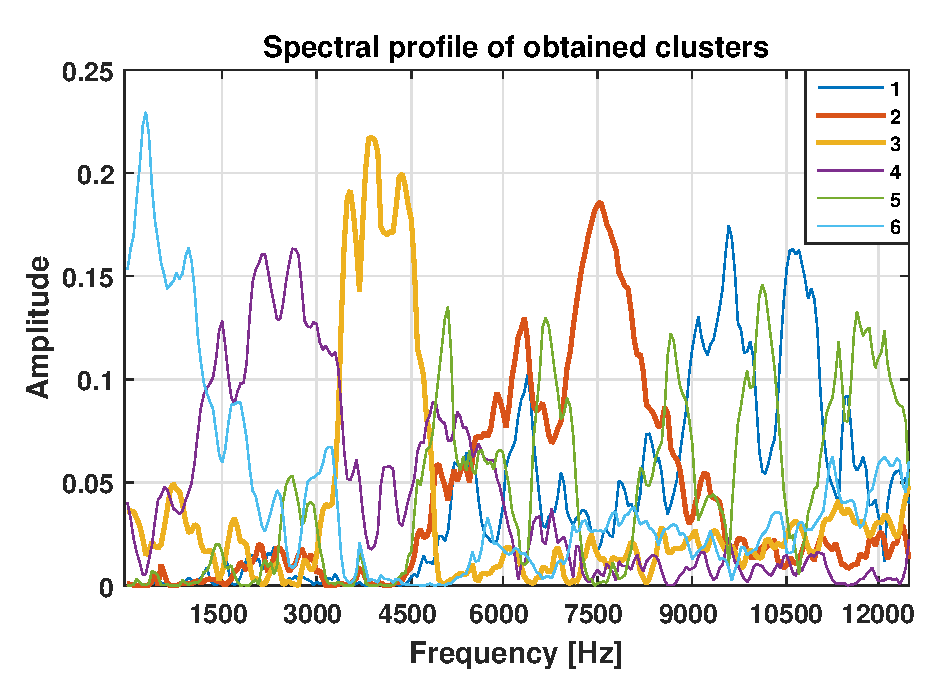
\includegraphics[width = 0.7\textwidth]{figs3/filt.eps}
\caption{Plot of IFB selectors for detected components for the ore crusher}
\label{fig: filt2}
\end{figure}

After evaluating kurtosis value of signals produced by filtering input signal with each obtained filter, 2 components with greatest values (produced by filters 2 and 3) are selected for final evaluation. Fig. \ref{fig: out2} shows the results of filtration. 

\begin{figure}[!ht]
\centering
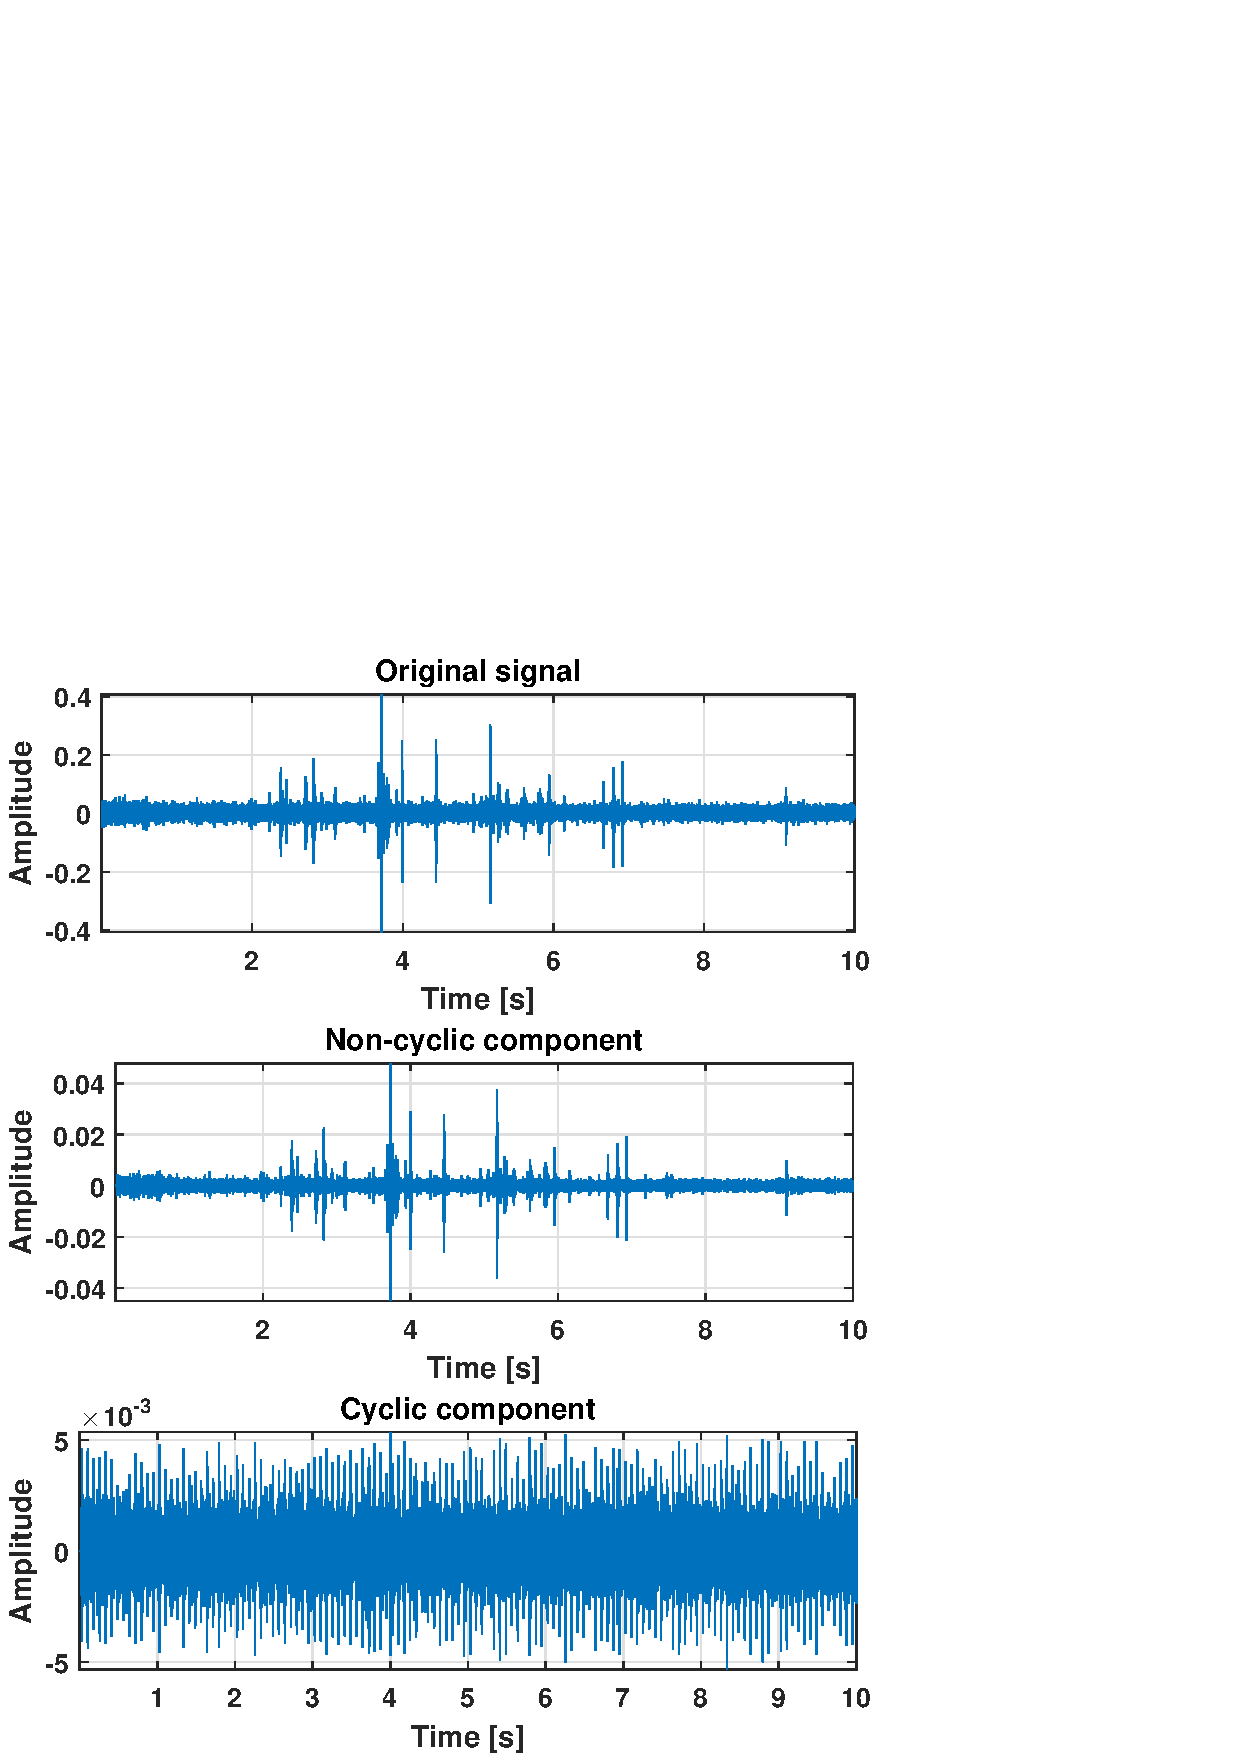
\includegraphics[width = 0.7\textwidth]{figs3/out.png}
\caption{Results of filtration for the ore crusher. Top: original signal, middle: non-cyclic component, bottom: cyclic component}
\label{fig: out2}
\end{figure}

As one can see, in case of input signal the damage is not visible either in the time series (Fig. \ref{fig: out2} top), or in the envelope spectrum (Fig. \ref{fig: widma2} top). It is very clear that overwhelming fraction of the signal information content is occupied by non-cyclic impulses as well as background components, since time series as well as envelope spectrum look almost exactly the same for input signal and for extracted non-cyclic component (see Fig. \ref{fig: out2} and \ref{fig: widma2} middle). 

On the other hand, initially invisible damage component is successfully extracted (Fig. \ref{fig: out2} bottom) and its envelope spectrum reveals clear information about the fundamental and harmonic frequencies of the damage. IFB determined for this component spans the frequencies between 3370 Hz and 4736 Hz of the carrier.

\begin{figure}[!ht]
\centering
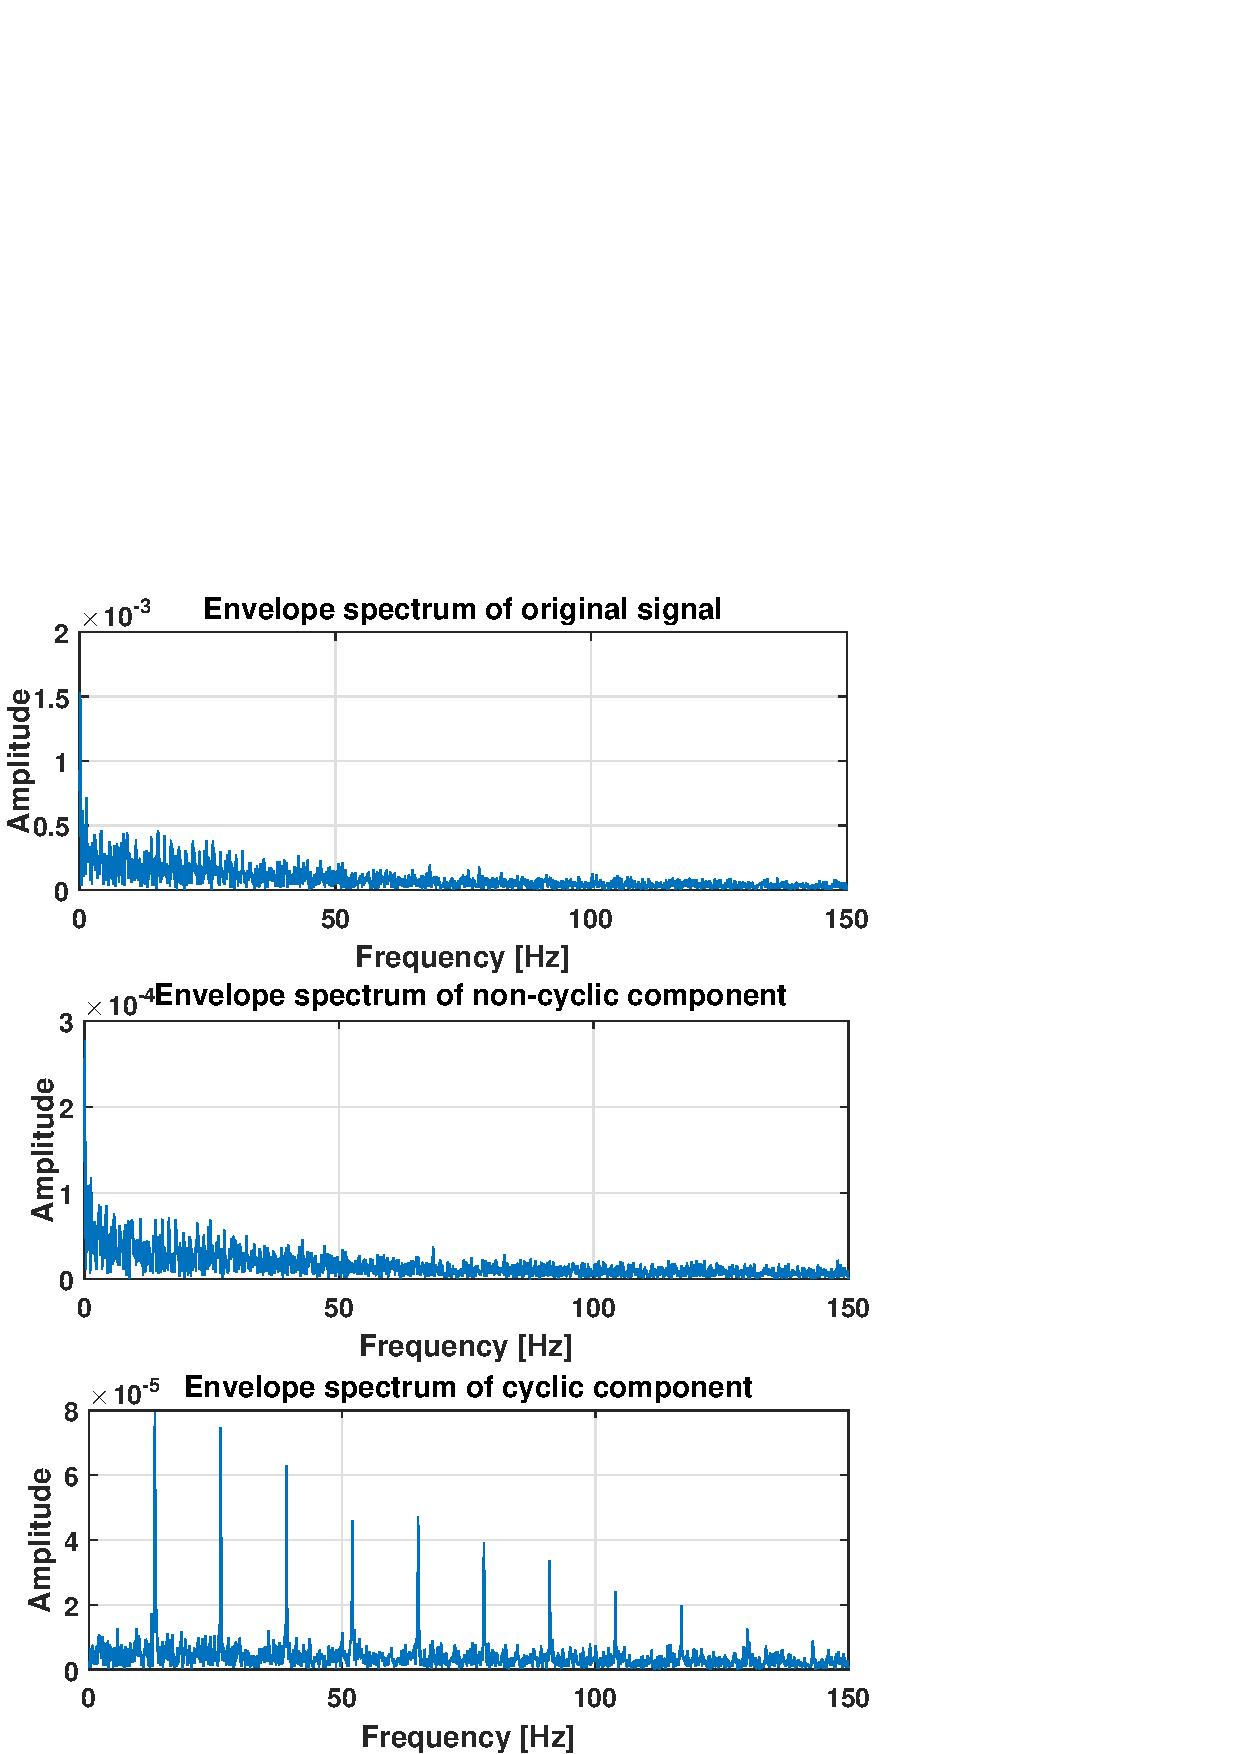
\includegraphics[width = 0.6\textwidth]{figs3/widma.png}
\caption{Envelope spectra of the results for the ore crusher: a) original signal, b) non-cyclic component, c) cyclic component}
\label{fig: widma2}
\end{figure}

\section{Conclusion}


In this paper authors introduce a novel approach to local damage detection in rotating machinery. It is proposed to perform Nonnegative Matrix Factorization of the spectrogram matrix. NMF is used as clustering tool here for spectral content with respect to time domain. After factorisation (approximation of input matrix V - i.e. spectrogram - by multiplication of two matrices W and H)  we consider base matrix W as a set of averaged - for given cluster - spectral characteristics. We call them "selector bank" because each of them might select some spectral content from raw signal. These characteristics might be used as filter characteristic that allow to extract part of the signal that belongs to given cluster and carries information about source signal. In our case 3 the most important clusters are: noise only, cyclic impulsive contribution, non-cyclic impulsive contribution. It is worthy to note that for noise component IFB doesnt exist - characteristic is rather flat. For two other impulsive sources amplitudes in the characteristics have significant higher level at some specific frequency ranges - recognised as IFB. Drawback of this method is the fact that multiple components cannot lie in entirely overlapping frequency bands - in such a case NMF will locate them into the same cluster. Method has been succesfully walidated using simulated and real data.

% conference papers do not normally have an appendix

% use section* for acknowledgment
% \section*{Acknowledgment} RockVader
% This work is partially (J. Wodecki, P. Kruczek, A. Wy{\l}oma{\'n}ska) supported by the Framework Programme for Research and Innovation Horizon 2020 under grant agreement n. 636834 (DISIRE -Integrated Process Control based on Distributed In-Situ Sensors into Raw Material and Energy Feedstock) 

% The work is supported by the Statutory Grant (Rados{\l}aw Zimroz)
\section*{References}
% \bibliographystyle{IEEEtran}
\bibliography{mybib}

\end{document}